%==============================================================================
\chapter{Neural Network Setup}
\label{sec:NNSetup}
%==============================================================================

Before the Neural Networks introduced in Chapter \ref{sec:ANNs} can be used to analyze the datasets described in Chapter \ref{sec:Samples}, the data needs to be prepared. The preprocessing involves the definition of a dataset splitting strategy to properly treat overfitting and the selection of representative input features for both FNNs and RNNs. Moreover, the transformation of the input features and renormalization of the event weights. \\
For the practical implementation of Neural Networks, the API Keras with Tensorflow as a backend is used throughout this thesis. 


\section{Splitting Strategy}
\label{sec:splitting}

\begin{figure}[H]
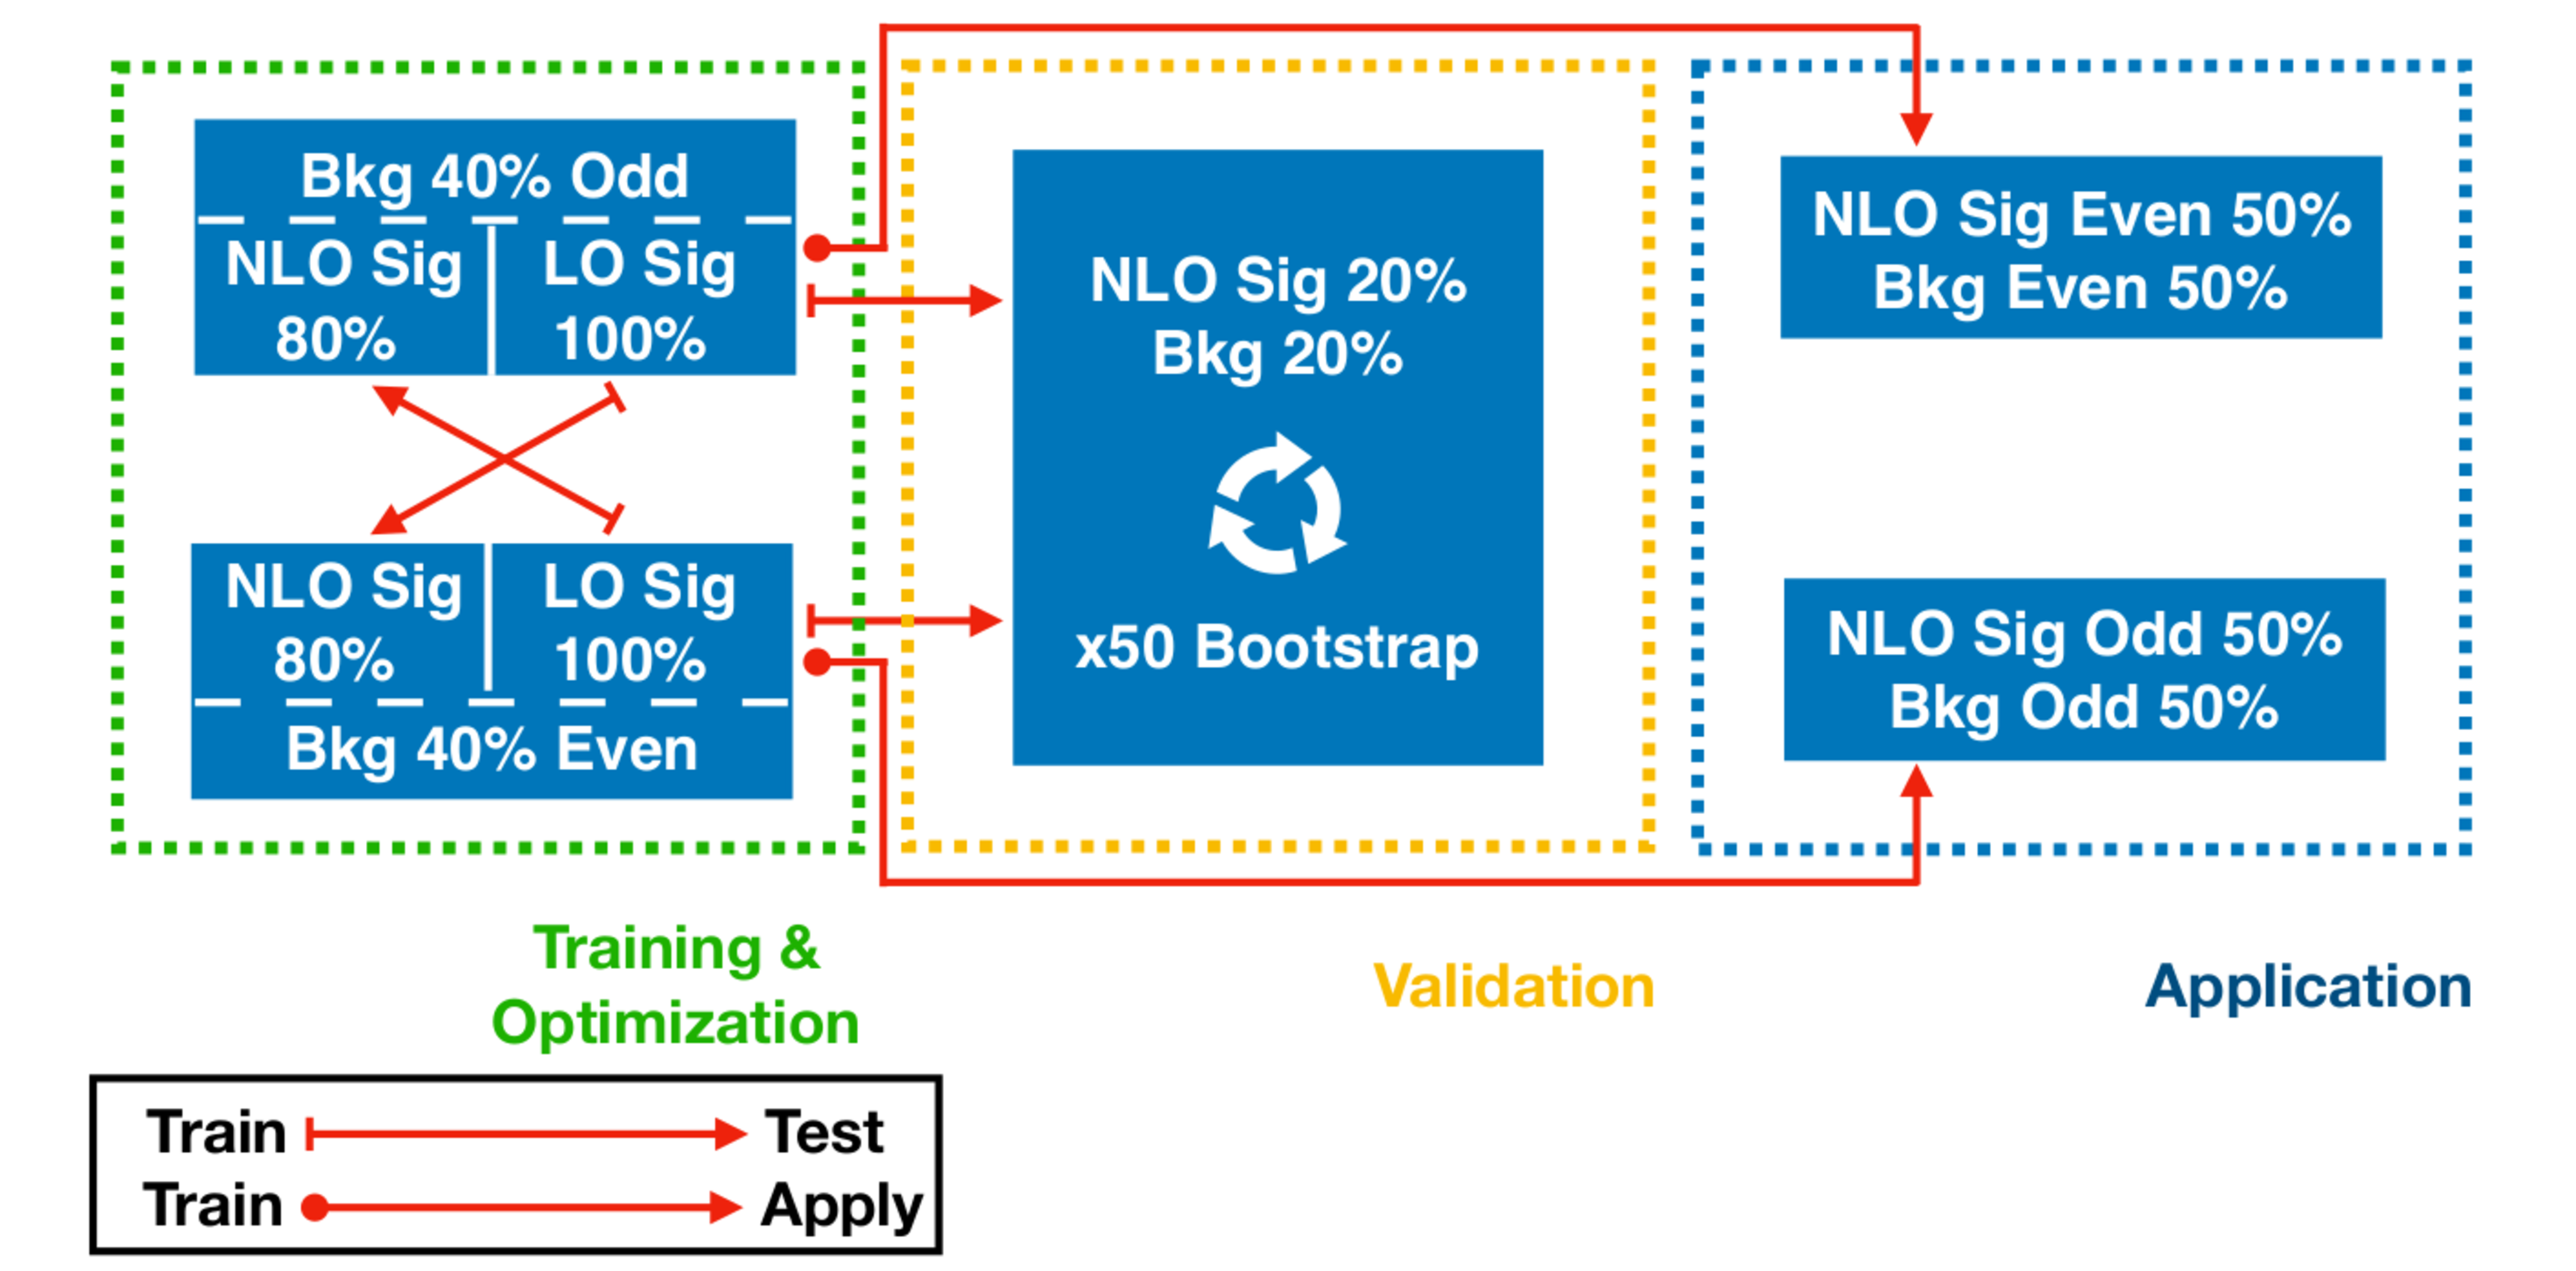
\includegraphics[width=\linewidth , left]{figs/splitting.pdf}
\caption{Splitting strategy that is applied to ensure unbiased estimation of both overtraining and performance. (plot by \"O O\u{g}ul Oncel)}
\label{fig:splitting}
\end{figure}

The two essential quantities of every machine learning model are the performance measure and its overtraining. As discussed in Section \ref{sec:optimization} the performance measure of choice is the AUC ($\Gamma$). It can be evaluated on a single dataset. Overtraining, however, measures how well a model trained on one dataset generalizes to a second dataset. Thus, at least two datasets are needed to evaluate the overtraining of a model. An important side note is that the two datasets need to be orthogonal i.e. they do not have events in common. Therefore, the original dataset is split into two independent datasets called the \textit{training} and the \textit{testing dataset}. As the name suggests, the training of the Neural Network is performed on the training dataset. After all trainable parameters are fixed, the model is tested on the testing dataset. The overtraining $O_v$ as a function of the two obtained AUCs $\Gamma_{\text{test}}$ and $\Gamma_{\text{train}}$ can be expressed as
\begin{equation}
O_v = 1 - \frac{\Gamma_{\text{test}}}{\Gamma_\text{train}}
\label{eq:overtraining}
\end{equation}
The Neural Network with the highest AUC, which has a reasonable $O_v$, typically under 5\%, is considered the best model. The detailed strategy to discover the best model is described in chapter \ref{sec:Results}. The optimization relies on training numerous models with different hyperparameters and architectures. However, since the same testing dataset is exploited multiple times, this approach introduces a bias into the overfitting measurement. To compensate for this, a third orthogonal dataset called the \textit{validation dataset} is introduced. Similar to the testing dataset, it is spared during training and additionally also remains unused during the optimization. Only after all hyperparameters are fixed, the $\Gamma_{\text{validation}}$ is calculated. Thus, allowing for unbiased estimation of $O_v$. Equation \ref{eq:overtraining} needs to be adjusted by replacing $\Gamma_{\text{test}}$ with $\Gamma{\text{validation}}$, for the final evaluation of the overtraining. The error of the obtained overfitting is then evaluated by generating multiple versions of the validation dataset and evaluating the AUC on all of them. The different versions of the validation dataset are generated using random sampling with replacement referred to as \textit{bootstrapping}. \\
The background datasets available of the four-top-quark analyses are split into 20\% validation dataset and 80\% for testing and training. The segmentation of the dataset containing 80\% of all background events is performed by splitting on the event number\footnote{The event number is the position of the event in the dataset.} (even or odd). The obtained datasets are referred to as the \textit{even} and the \textit{odd dataset}. This procedure is applied for each background dataset individually such that the three final datasets have a proper number of events for each process. The $t\bar{t}t\bar{t}$ signal dataset, since it holds events calculated both at leading order and next-to-leading order, is treated differently. All LO events are used for training to avoid the negative event weights problem, which will be discussed in section \ref{sec:transformation}. The NLO events are split into 80\% testing dataset and 20\% for validation dataset. The complete splitting strategy is summarized in Figure \ref{fig:splitting}. The application step indicated corresponds to further studies of the $t\bar{t}t\bar{t}$ process performed on the NLO events. As the red arrows imply, two Neural Networks with the same hyperparameters are trained. The first one uses the even dataset as the training dataset and the odd dataset as the testing dataset (yielding $\Gamma_{\text{even}}$). The definition of the testing and training dataset is interchanged for the second Neural Network (yielding $\Gamma_{\text{odd}}$). The combined AUC $\Gamma_{\text{total}}$ can be determined as
\begin{equation}
\Gamma_{\text{total}} = \frac{\Gamma_{\text{even}} + \Gamma_{\text{odd}}}{2}
\end{equation}
This scheme ensures that the final performance measure $\Gamma_{\text{total}}$ is independent of the concrete choice of the training and testing datasets. 

\section{Feature Selection}
\label{sec:feature_selection}

The selection of input features is crucial to obtain a Neural Network with a high AUC. The features selected have to discriminate the signal process well from the background processes. If to many or irrelevant features are selected, the training of the Neural Network is slow down which in turn can lead to decreased performance. The usage of prior information about the problem, such as the different physical characteristics of a processes, can be used as a guideline to find good separating features. In the case of the $t\bar{t}t\bar{t}$ process,
it is known that the final state has a high jet and b-jet multiplicity (cf. Section \ref{sec:fourtops}). As can be seen in Figures \ref{fig:MV2c10} to \ref{fig:dRbb} these properties are reflected in the number of jets ($n_{j}$) and the b-tagging score $\sum w_{\text{MV2c10}}$. To be more precise $\sum w_{\text{MV2c10}}$ is calculated by assigning each jet in the event a weight depending on its MV2c10 score. The weights can take values between 1, if the jet passes non of the working points, and 5, if jet passes all of the working points. \\
In practice, resolution and detector effects can smear out expected characteristics. Therefore, it is necessary to validate which features increase $\Gamma_{\text{total}}$. As the first figure of merit, the ranking of features provided by a boosted decision tree \cite{BDT} is adopted. The ranking is derived by counting how often a feature is used to split decision tree nodes, and by weighting each split occurrence by the separation gain squared, it has achieved \cite{TMVA}. To ensure that the highest-ranking features are also well suited for Neural Networks, a study using an iterative removal algorithm is performed. This algorithm aims to find the best $k$ features out of a set of $m$ features, by training $m$ Neural Networks with the same hyperparameters. Each of the Neural Networks is trained without one of the $m$ features. The feature that had the least impacted on the AUC is removed. This process is repeated until only $k$ features remain.
The 18 features selected in this manner are summarized in table \ref{tab:feature_selection}, together with the respective BDT ranking scores. As previously mentioned, $N_j$ and $\sum w_{\text{MV2c10}}$ are two of the highest-scoring features alongside the angular distance features $\Delta R(x,y)$ which are calculated according to
\begin{equation}
\Delta R(x,y) = \sqrt{(\eta_x - \eta_y)^2 + (\phi_x - \phi_y)^2}
\end{equation}
where x and y are two particle types. An example of an angular distance distribution is shown in Figure \ref{fig:dRbb}. $\Delta R(b,b)_{\text{min}}$ refers to the minimum angular distance between any b-jet pair. \\

\begin{table}[H]
\begin{tabular}{|l|l|l|}
\toprule
Feature & Definition & BDT ranking score \\
\midrule \midrule
$\sum w_{\text{MV2c10}}$ & Sum of b-tagging weights of MV2c10 & 0.114 \\
$\Delta R(l,l)_{\text{min}}$ & Maximum angular distance between any lepton pair & 0.063 \\
$p_{\text{T}}^{j,0}$ & $p_{\text{T}}$ of the leading jet & 0.063 \\
$E_{\text{T}}^{\text{miss}}$ & missing transverse energy & 0.059 \\
$N_j$ & Jet multiplicity & 0.059 \\
$p_{\text{T}}^{\ell,0}$ & $p_{\text{T}}$ of the leading lepton & 0.059 \\
$p_{\text{T}}^{b,0}$ & $p_{\text{T}}$ of the leading b-jet & 0.058 \\
$\Delta R(b,b)_{\text{min}}$ & Minimum angular distance between any b-jet pair & 0.055 \\
$p_{\text{T}}^{j,5}$ & $p_{\text{T}}$ of the fifth highest jet & 0.055 \\
$\Delta R(l,b)_{\text{max}}$ & Maximum angular distance between any lepton and b-jet & 0.054 \\
$\Delta R(l,j)_{\text{min}}$ & Minimum angular distance between any lepton and jet & 0.051 \\
$H_{\text{T}}^{0}$ & Scalar sum of all lepton and jet $p_{\text{T}}$'s excluding the leading jet & 0.049 \\
$p_{\text{T}}^{\ell,1}$ & $p_{\text{T}}$ of the sub-leading lepton & 0.049 \\
$\sum_l \Delta R(l,l)$ & Sum of all angular distance between any lepton pair & 0.040 \\
$p_{\text{T}}^{j,1}$ & $p_{\text{T}}$ of the sub-leading jet & 0.039 \\
$\Delta R(l,l)_{\text{max}}$ & Maximum angular distance between any lepton pair & 0.039 \\
$\Delta R(l,b)_{\text{min}}$ & Minimum angular distance between any lepton and b-jet & 0.039 \\
$\phi^{\ell,0}$ & $\phi$ of the leading lepton & 0.038 \\
\bottomrule
\end{tabular}
\caption{The 18 selected features for the FNNs with there respective BDT ranking score}
\label{tab:feature_selection}
\end{table}


The approach chosen to select features for the RNN is different and is loosely inspired by \cite{RNNSel}. The four momenta and the decaying angles of the reconstructed objects in the final state are used directly as input features. If multiple particles of the same type are present in the final state of an event, this particles are sorted according to their $p_{\text{T}}$. Thus, an input feature such as the pseudorapidity of any jet $\eta_j$ is a $p_{\text{T}}$ sorted sequence of length $N_j$ where $n_j$ is the number of jets observed in the event.  In practice, all input feature sequences in the same event have to have the same length. This is accomplished by padding sequences that do not have the desired length with zeros. In addition to the features described above, some high-level features, such as $\sum w_{\text{MV2c10}}$, are selected. The combination of the two types of features was shown to increase performance in several applications \cite{SpeFea1,SpeFea2}. The input features selected are $\phi$, $\eta$, $p_{\text{T}}$ of electron, muons and jets as well as $E_{\text{T}}^{\text{miss}}$, $\phi_{\text{T}}^{\text{miss}}$, $N_j$ and $\sum w_{\text{MV2c10}}$. All features for FNNs and RNNs are shown in detail in the Appendix \ref{ap:Input}.

\newpage

To have some kind of feature selection, a small $\ell$1 regularization term is applied to the RNN. As briefly mentioned in Section \ref{sec:optimization}, this regularization tends to eliminate connections to the least important features. Thus an automatic feature selection is provided, which suppresses redundant information.

%\begin{figure}[H]
%\begin{minipage}[t]{.5\linewidth}
%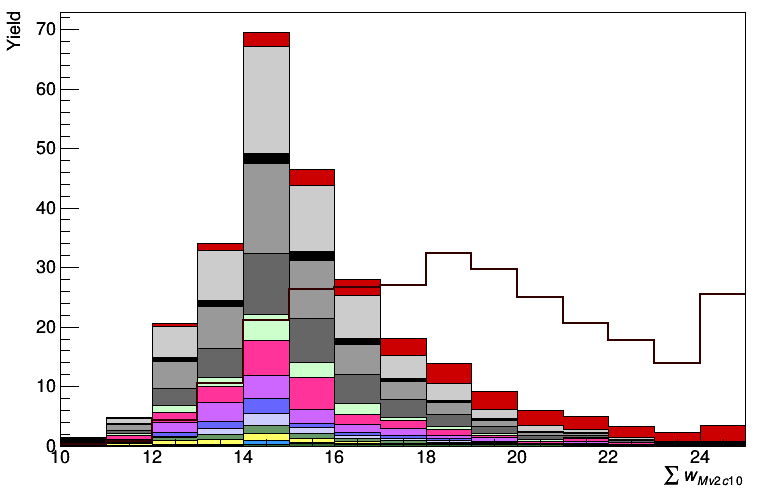
\includegraphics[width=\linewidth]{figs/features/MV2c10.png}
%\caption{Sum of the continuous MV2c10 b-tagging score}
%\label{fig:MV2c10}
%\end{minipage}
%\hspace{.01\linewidth}
%\begin{minipage}[t]{.5\linewidth}
%\includegraphics[width=\linewidth]{figs/features/nJets.png}
%\caption{Jet multiplicity}
%\label{fig:nJets}
%\end{minipage}
%
%
%\begin{minipage}[t]{.5\linewidth}
%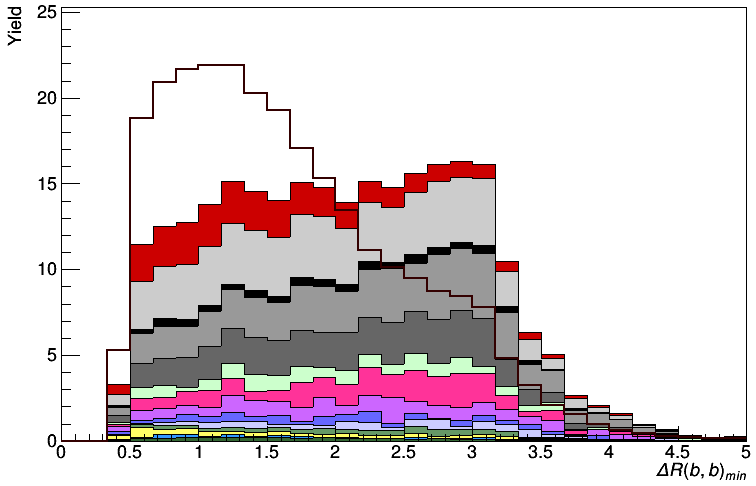
\includegraphics[width=\linewidth]{figs/features/dRbbmin.png}
%\caption{minimum angular distance between any b-jet pair}
%\label{fig:dRbbmin}
%\end{minipage}
%\hspace{.01\linewidth}
%\begin{minipage}[t]{.5\linewidth}
%\centering
%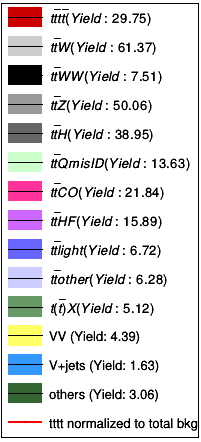
\includegraphics[width=0.3\linewidth]{figs/features/legende.png}
%\caption{Legend}
%\label{fig:Legend}
%\end{minipage}
%
%\end{figure}


\begin{figure}[H]
\begin{subfigure}{.5\textwidth}
  \centering
  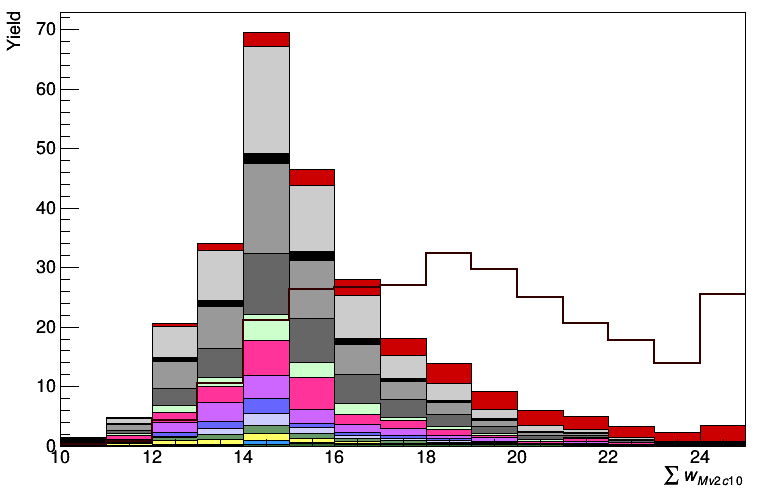
\includegraphics[width=.99\linewidth]{figs/features/MV2c10}
  \caption{Sum of b-tagging weights of MV2c10}
  \label{fig:MV2c10}
\end{subfigure}%
\begin{subfigure}{.5\textwidth}
  \centering
  \includegraphics[width=.99\linewidth]{figs//features/nJets}
  \caption{Jet multiplicity}
  \label{fig:nJets}
\end{subfigure}
\begin{subfigure}{.5\textwidth}
  \centering
  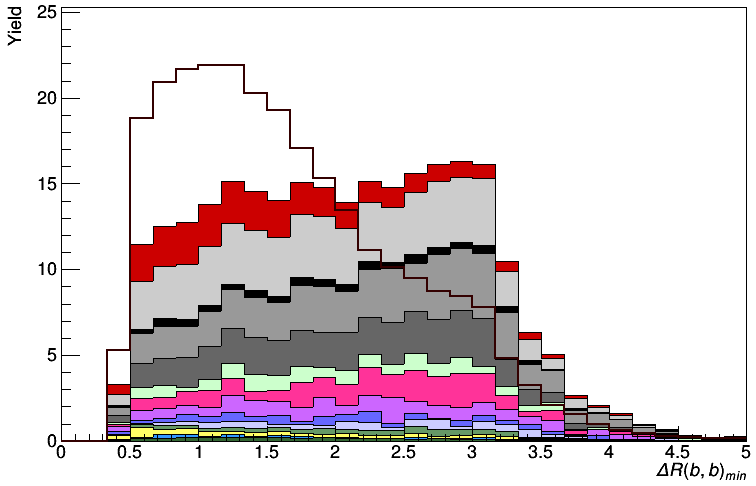
\includegraphics[width=.99\linewidth]{figs/features/dRbbmin}
  \caption{minimum angular distance between any b-jet pair}
  \label{fig:dRbb}
\end{subfigure}%
\begin{subfigure}{.5\textwidth}
  \centering
  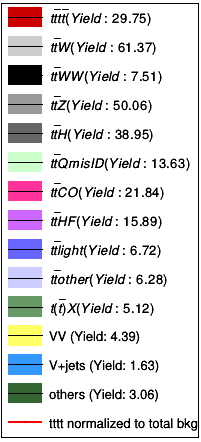
\includegraphics[width=.29\linewidth]{figs/features/legende}
  \caption{Legend}
  \label{fig:LegendwY}
\end{subfigure}
\caption{Three of the most discriminating features of the FNN study. The last bin in all distribution contains additionally the events which fall into bins above the maximum x-axis range.}
\label{fig:BestFeatures}
\end{figure}


\section{Feature Transformation and Event Weight Treatment}
\label{sec:transformation}

As discussed in Section \ref{sec:training}, the backpropagation algorithm calculates the gradients of the loss function for each weight, starting from the output layer and working backward to the input layer. Each gradient of the current step, therefore, depends on the gradients derived in the previous step. Thus, when the selected input features have small numerical values, the gradients start to \textit{vanish} \cite{MainNN}, leaving the weights virtually unchanged. On the other hand, if the features have big numerical values, the gradients can become very large, leading to the \textit{exploding gradient problem} \cite{MainNN}. Both cases can hinder the convergence of the Neural Network. One way of dealing with this problem is to transform all input features to normal distributions i.e. 0 mean and a variance of 1, before feeding them to the Neural Network. This transformation is crucial. Neural Networks trained without it show an up to 0.2 decreased AUC compared to the same Neural Networks with transformed input features. Additionally, the SELU activation function can be utilized to normalize the neuron outputs at each layer.\\

\begin{figure}[H]
\begin{subfigure}{.5\textwidth}
  \centering
  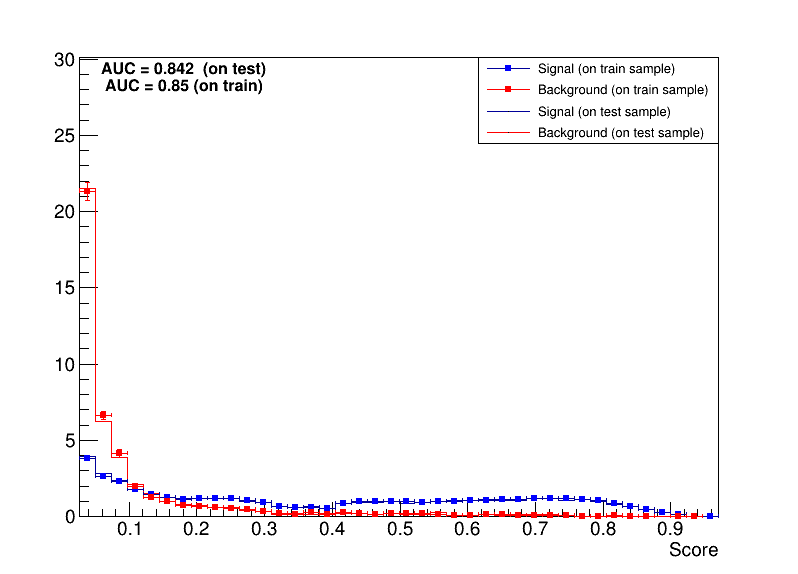
\includegraphics[width=.99\linewidth]{figs/Score_w_weights}
  \caption{Event weights applied}
  \label{fig:ScoreWeights}
\end{subfigure}%
\begin{subfigure}{.5\textwidth}
  \centering
  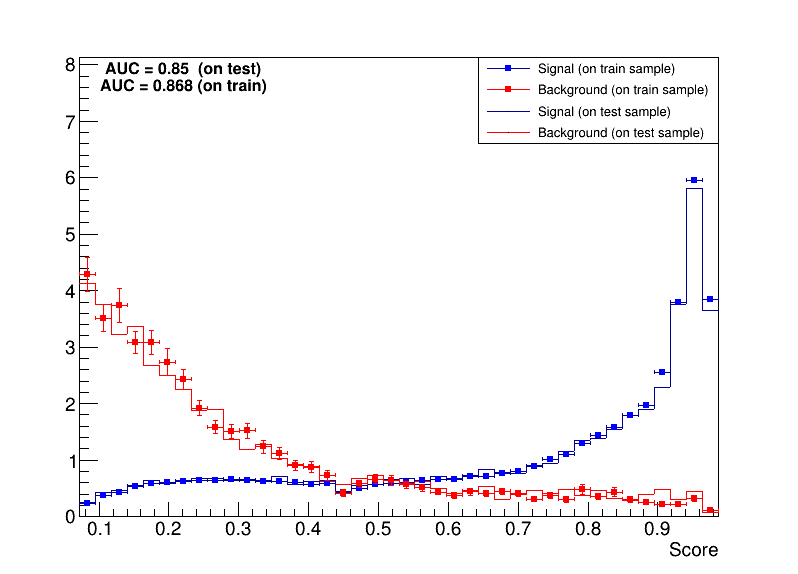
\includegraphics[width=.99\linewidth]{figs/Score_reweighted}
  \caption{Renormalization event weights applied}
  \label{fig:ScoreRenormed}
\end{subfigure}
\caption{The difference in classification between a Neural Network trained with and without renormalization event weights.}
\label{fig:ScoreWvsR}
\end{figure}

Event weights are interpreted as probabilities in Neural Networks. This probabilities are multiplied with the loss function at each training step.
When the event weights, introduced in Chapter \ref{sec:EventSelection}, are very small or very large, the he training of Neural Networks are effect by the vanishing and exploding gradient problem. This is because gradients are calculated based on the loss function. To avoid very large and very small event weights, a renormalization is applied such that the sum of all weighted signal training events equals the sum of all weights of the background training events, following the approach described in \cite{TMVA}. The renormalized event weight are exclusively used during training. \\
The score distributions\footnote{The y-axis of the displayed distributions shows the number of events normalized to $\frac{dN}{dx}$ where $dN$ is the total number of events and $dx$ is given by one over the number of bins.} shown in Figure \ref{fig:ScoreWvsR} are the probabilities assigned by the Neural Network for a given event to be a signal event. The red dots and lines represent events that truly originate from $t\bar{t}t\bar{t}$ events, while the blue dots and lines represent events that truly originate from background processes. The solid lines denote the score obtained for the training dataset while the dots denote the score obtained on the testing dataset. A perfect classifier would be a classifier for which all signal events are in the first bin, and all background events are in the last bin. \\
Figure \ref{fig:ScoreWeights} shows the score of a Neural Network trained without the renormalization applied. The Neural Network focuses on the background events since the total background Yield (228) is much higher than the signal Yield (30). The same Neural Network is used to obtain the score shown in Figure \ref{fig:ScoreRenormed}, the only difference being the applied renormalization of the weights. The classification with renormalization weights clearly separates background and signal events and ultimately results in an higher AUC. \\
 All negative events weights are set to 0 during the training since the usual interpretation of the event weight as probabilities can not be applied. A problem referred to as the \textit{negative weight problem} \cite{nWeights}.